% Source: Code/ML_overlay/ir_rgb_registration/paper/ml_overlay_report_materials/ir_rgb_registration_report/figures/fig_experiment_pipeline.tex
\documentclass[tikz,border=10pt]{standalone}
\usepackage{tikz}
\usetikzlibrary{positioning,shapes.arrows}

\definecolor{Garnet}{RGB}{115,0,10}
\definecolor{Rose}{RGB}{204,46,64}
\definecolor{Atlantic}{RGB}{70,106,159}
\definecolor{Congaree}{RGB}{31,65,77}
\definecolor{Horseshoe}{RGB}{101,120,11}
\definecolor{Black90}{RGB}{54,54,54}
\definecolor{White}{RGB}{255,255,255}

\begin{document}
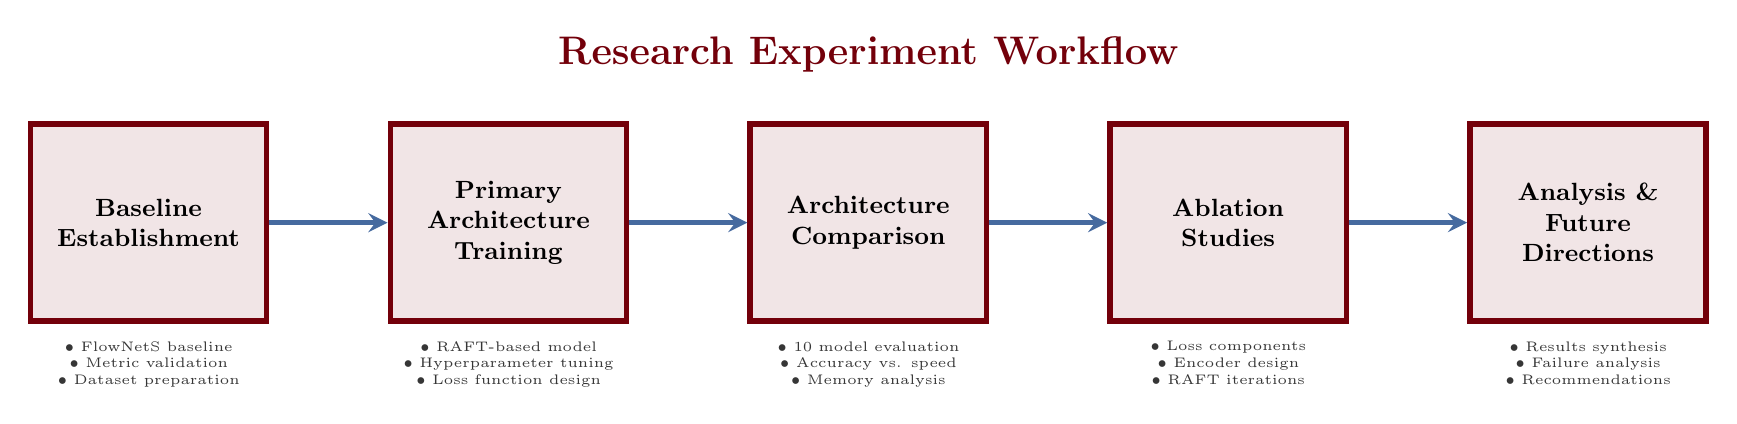
\begin{tikzpicture}[
    box/.style={rectangle,draw=Garnet,line width=2pt,fill=Garnet!10,
                minimum width=3cm,minimum height=2.5cm,align=center,font=\small\bfseries},
    arrow/.style={->,>=stealth,line width=2pt,Atlantic},
    subtitle/.style={font=\tiny,text width=2.8cm,align=center,Black90}
]

% Stage 1: Baseline Establishment
\node[box] (stage1) at (0,0) {Baseline\\Establishment};
\node[subtitle,below=0.1cm of stage1.south,anchor=north] (sub1) {
    $\bullet$ FlowNetS baseline\\
    $\bullet$ Metric validation\\
    $\bullet$ Dataset preparation
};

% Stage 2: Primary Architecture Training
\node[box,right=1.5cm of stage1] (stage2) {Primary\\Architecture\\Training};
\node[subtitle,below=0.1cm of stage2.south,anchor=north] (sub2) {
    $\bullet$ RAFT-based model\\
    $\bullet$ Hyperparameter tuning\\
    $\bullet$ Loss function design
};

% Stage 3: Architecture Comparison
\node[box,right=1.5cm of stage2] (stage3) {Architecture\\Comparison};
\node[subtitle,below=0.1cm of stage3.south,anchor=north] (sub3) {
    $\bullet$ 10 model evaluation\\
    $\bullet$ Accuracy vs. speed\\
    $\bullet$ Memory analysis
};

% Stage 4: Ablation Studies
\node[box,right=1.5cm of stage3] (stage4) {Ablation\\Studies};
\node[subtitle,below=0.1cm of stage4.south,anchor=north] (sub4) {
    $\bullet$ Loss components\\
    $\bullet$ Encoder design\\
    $\bullet$ RAFT iterations
};

% Stage 5: Analysis & Future Directions
\node[box,right=1.5cm of stage4] (stage5) {Analysis \&\\Future\\Directions};
\node[subtitle,below=0.1cm of stage5.south,anchor=north] (sub5) {
    $\bullet$ Results synthesis\\
    $\bullet$ Failure analysis\\
    $\bullet$ Recommendations
};

% Arrows connecting stages
\draw[arrow] (stage1.east) -- (stage2.west);
\draw[arrow] (stage2.east) -- (stage3.west);
\draw[arrow] (stage3.east) -- (stage4.west);
\draw[arrow] (stage4.east) -- (stage5.west);

% Title
\node[font=\Large\bfseries,Garnet,above=0.5cm of stage3.north] {Research Experiment Workflow};

\end{tikzpicture}
\end{document}
